\chapter{Descrição do Hardware} \label{chap:descricao_hard}

Nesse capítulo serão descritos elementos do hardware do robô DORIS associados ao funcionamento do manipulador TETIS. A descrição completa dos dispositivos do DORIS, pode ser obtida em \citep{xaud2016doris, nunes2013doris, freitas2015embedded, galassi2014doris}.

\section{Eletrônica Embarcada}

A eletrônica embarcada é composta de um computador central e subsistemas de comunicação, atuação, aquisição de dados e o \textit{Vehicle Suport System (VSS)} \citep{freitas2015embedded}. 

No projeto do DORIS, o computador consite em um módulo PCIe/104 com Intel\circledR Core i7\texttrademark e disco de estado sólido (SSD). Atualmente ele está operando com um módulo PCIe/104 Intel\circledR Atom D525. 

O sistema de comunicação trata do tráfego de dados entre o robô e a base remota. É composto de:

\begin{itemize}
\item Rede Local \textit{Gigabit Ethernet}. È responsável pela comunicação de alta largura de banda entre o DORIS e seus diversos periféricos. A essa rede estão conectados o computador embarcado, cameras \textit{Ethernet}, access points Wi-Fi, roteadores, o \textit{Vehicle Support System} (VSS).
\item \textit{Controller Area Network (CAN)}. É responsável pelo controle em tempo real do sistema de atuação através de uma rede robusta. A rede CAN integra os drivers do sistema de atuação e os computadores embarcados em uma topologia de rede em barramento. 

\item Tecnologias sem fio: O DORIS pode ser remotamento operado por meio de rede \textit{Wi-Fi IEEE 802.11m} ou através de um rádio 2.4/5.0 GHz caso ocorra alguma falha na conexão.
\end{itemize}

O sistema de aquisição de dados coleta imagem, video e áudio do ambiente. É composto de uma camera fixa, uma câmera térmica, uma câmera \textit{fish-eye}, duas câmeras estereoscópicas e uma unidade de medição inercial (IMU).

\section{Atuadores e Drivers}

O sistema de atuação é responsável pela atuação dos motores do DORIS. É composto pelo subsistema de tração e pelo subsistema do manipulador. As juntas de revolução do TETIS necessitam de atuadores com as seguintes características:

\begin{itemize}
\item Alto taxa de redução, para permitir controle a nível de velocidade nas juntas.
\item Folga desprezível, para evitar a adição de não linearidades ao sistema. 
\item Eixo oco para permitir o roteamento de cabos através dele.
\item Alta acurácia e repetibilidade
\end{itemize}

A tecnologia \textit{Harmonic gear}, registrada pela \textit{Harmonic Drive}, consiste em engrenagens do tipo \textit{strain wave}. Esse mecanismo melhora certas características em comparação com sistemas de transmissão tradicionais como engrenagens helicoidais, ou planetárias. As vantagens incluem a inexistência de folgas, mais compacto, leve, altas taxas de redução, excelente resolução e repetibilidade e alto torque.

As juntas do manipulador TETIS utilizam atuadores \textit{FHA Mini Servo} da \textit{Harmonic Drive AG}, mostrados na figura \ref{fig:harmonic_drive}. Segundo o estudo em \citep{xaud2016doris}, esse atuador cumpre os requisitos acima. Ele conta também com \textit{encoder}, montado no eixo do motor, antes da redução, e sensores \textit{hall} para os três enrolamentos. Com base nos requisitos de torque, para as duas primeiras juntas é utilizado o modelo FHA-11C-100-D200-EKMI, enquanto que para as duas últimas o modelo FHA-8C-100-D200-EKMI.

\newlength{\twosubht}
\newsavebox{\twosubbox}

\begin{figure}[htp]
% preliminary
\sbox\twosubbox{%
  \resizebox{\dimexpr.9\textwidth-1em}{!}{%
    \includegraphics[height=3cm]{./img/fha-c_mini.jpg}%
    \includegraphics[height=3cm]{./img/epos2-70-10.png}%
  }%
}
\setlength{\twosubht}{\ht\twosubbox}
% typeset
\centering
\subcaptionbox{Harmonic Drive FHA Mini Servo\label{f}}{%
  \includegraphics[height=\twosubht]{./img/fha-c_mini.jpg}%
}\quad
\subcaptionbox{Maxon Motor EPOS2 70/10\label{s}}{%
  \includegraphics[height=\twosubht]{./img/epos2-70-10.png}%
}
\caption{Atuadores e Drivers}
\end{figure}


Para atinjir um controle satisfatório a nível de junta, são utilizados drivers da Maxon Motor, compatíveis com o barramento CAN. Cada junta é controlada por um driver modelo Maxon Motor EPOS2 70/10 P/N 375711, mostrado na figura \ref{fig:epos}.

\section{Câmera Minoru} \label{sec:minoru}

O robô DORIS conta com diversos tipos de câmeras, como camera de alta definição, térmica, \textit{fisheye} e estereoscópica. 

A figura \ref{fig:efet_minoru} mostra a câmera utilizada para o controle por servovisão e o efetuador com a câmera montada.
A câmera em questão é a \textit{Minoru 3D Webcam}, uma câmera esterescópica que possui dois sensores VGA CMOS. É um dispositivo leve que pode ser acoplado ao efetuador final.

\begin{figure}[H]
\centering
\begin{subfigure}{.5\textwidth}
  \centering
  \includegraphics[width=0.75\linewidth]{./img/manip_zoom.png}
  \caption{Efetuador com câmera}
  \label{fig:efetuador}
\end{subfigure}%
\begin{subfigure}{.5\textwidth}
  \centering
  \includegraphics[width=0.6\linewidth]{./img/minoru.jpg}
  \caption{Minoru Camera}
  \label{fig:minoru}
\end{subfigure}
\label{fig:efet_minoru}
\caption{Efetuador e câmera Minoru}
\end{figure}

\section{Sensor de Força} \label{sec:optoforce}

No efetuador do manipulador TETIS há um sensor de força da \textit{OptoForce Kft.}, modelo OMD-20-FE-200N. Os sensores Optoforce 3D medem a magnitude e direção de forças $F_x$, $F_y$ e $F_z$ utilizando princípios ópticos \cite{optoforce}. O sensor utiliza uma interface USB. 

\begin{figure}[!ht]
\centering
  \includegraphics[width=\linewidth]{./img/optoforce.png}
  \caption{Optoforce OMD-20-FE-200N \cite{optoforce}}
  \label{fig:optoforce}
\end{figure}%

\begin{table}[h!]
\centering
\caption{Capacidade do sensor Optoforce OMD-20-FE-200N}
\label{tab:dh_tetis}
\begin{tabular}{lrr} \hline
 &  Capacidade Nominal & Deformação Típica \\ \hline
 $F_{xy}$ & $\pm 20N$ & $\pm 1.5 mm$ \\
 $F_z $ - Compressão & $200N$ & $1.2 mm$ \\
 $F_z $ - Tensão & $100N$ & $1 mm$ \\
\hline
\end{tabular}
\end{table}


\section{Integração dos dispositivos}

A malha de controle do manipulador TETIS é integrada através da \textit{Controller Area Network} (CAN) e da interface USB do computador embarcado PCIe/104. O computador é o nó principal, recebendo dados de sensores e enviando comandos de controle para os drivers.

Através da interface USB, o computador recebe realimentação do sensor de força e vídeo da câmera. A realimentação dos encoders é feita através do barramento CAN, passando pelos drivers EPOS2. A figura \ref{fig:integration} ilustra a integração do manipulador ao sistema do robô.

\begin{figure}[!ht]
\centering
  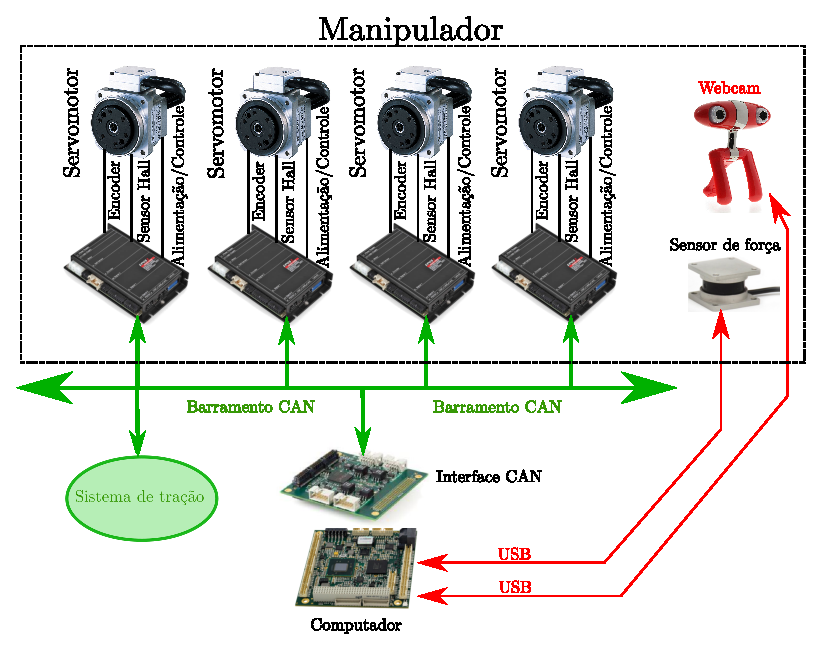
\includegraphics[width=\linewidth]{./img/integration_diagram}
  \caption{Esquema de integração dos dispositivos.}
  \label{fig:integration}
\end{figure}%